\section{Operazioni di configurazione delle impostazioni di collegamento}\label{PreMonitoraggio}
Questa sezione ha lo scopo di illustrare in dettaglio le operazioni che devono essere necessariamente svolte dall'utente prima di poter usufruire correttamente del monitoraggio dati (§\ref{Monitoraggio}).\\
Si tratta di operazioni necessarie alla definizione delle impostazioni di collegamento tra rete bayesiana e flusso dati.


\subsection{Caricamento di una Rete Bayesiana}\label{ReteB}

L'Operazione di caricamento della rete Bayesiana consta di due passaggi fondamentali:
\begin{enumerate}
	\item \textbf{Passaggio 1}: L'utente accede al pannello di selezione della rete bayesiana cliccando il pulsante \textbf{Upload .json file} presente in Figura \ref{Pannello};
	\item \textbf{Passaggio 2}: L'utente seleziona, tra i files presenti nella propria macchina, la rete bayesiana che desidera caricare e preme il pulsante \textbf{Apri} (Figura \ref{UploadRete}).
\end{enumerate} 

\begin{figure}[H]
	\begin{center}
		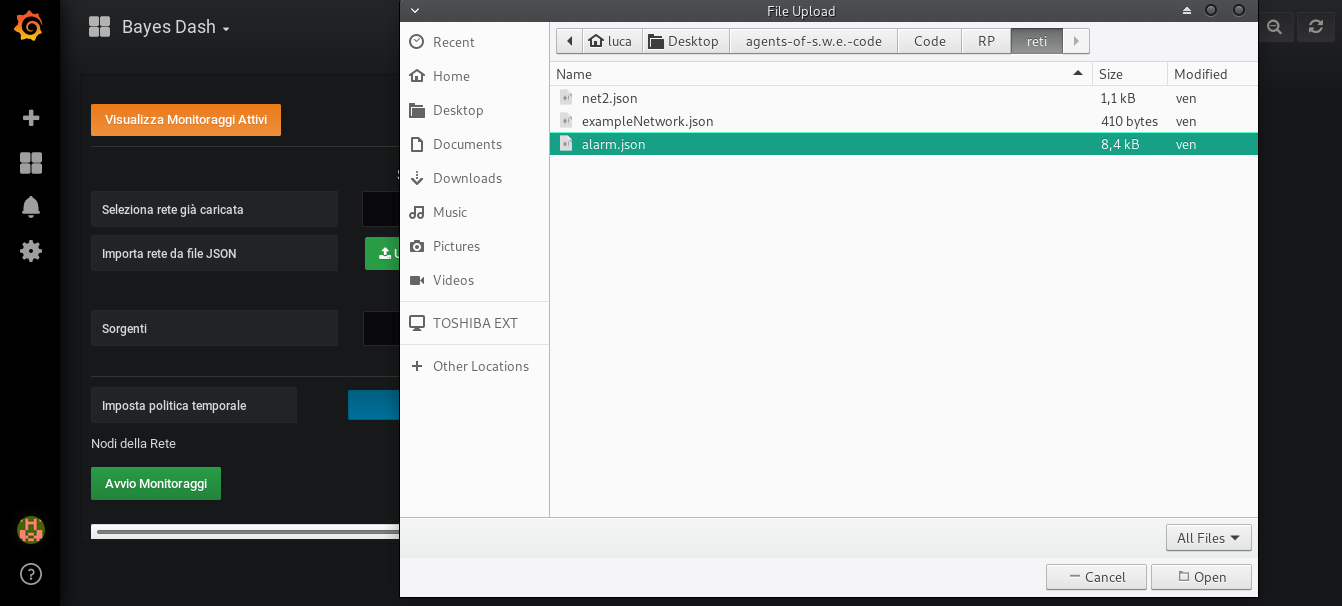
\includegraphics[scale=0.3]{./images/UpRete.png}
		 \caption{Pannello di caricamento Rete Bayesiana}	
		 \label{UploadRete}
	\end{center}
\end{figure}

L'estensione accettata dal plug-in per il file di definizione della rete è \textit{.json}. La rete bayesiana deve essere ben formata, seguendo le direttive della libreria \textit{JSBayes}. Inoltre la rete deve contenere un identificativo del proprio nominativo, necessario al momento del salvataggio della rete nel server.\\
~\\
Al seguito del corretto caricamento della rete bayesiana l'utente verrà avvisato del buon esito dell'operazione da un messaggio di notifica. Verrà inoltre visualizzato nel pannello \textit{G\&B} la lista dei nodi di cui è composta la rete bayesiana caricata (Figura \ref{NodiRete}).

\begin{figure}[H]
	\begin{center}
		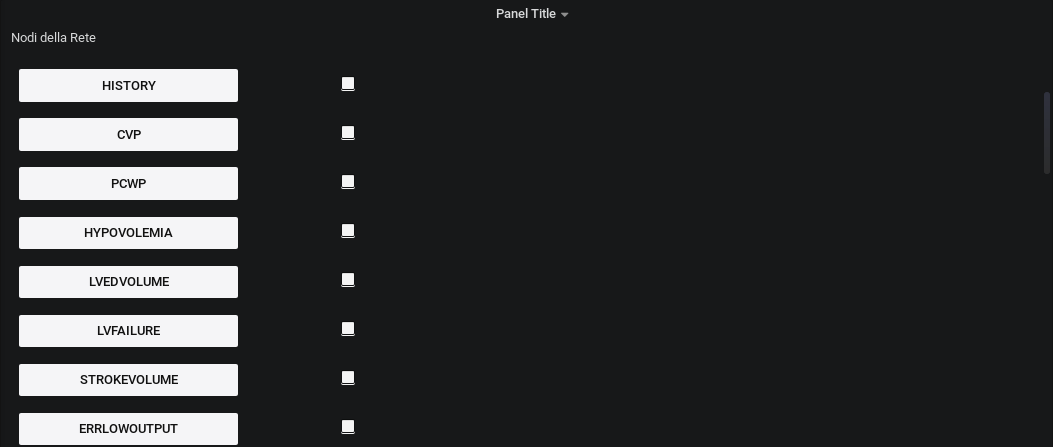
\includegraphics[scale=0.35]{./images/NodiRete.png}
		 \caption{Visualizzazione dei nodi della rete bayesiana caricata}	
		 \label{NodiRete}
	\end{center}
\end{figure}

Nel caso l'utente stesse visualizzando una diversa rete bayesiana prima del caricamento del nuovo file questa viene memorizzata nel server insieme alle sue eventuali impostazioni di collegamento.

~\\
\textbf{\textcolor{red}{ATTENZIONE}}: Nel caso in cui l'utente abbia selezionato per il caricamento un file di definizione della rete non conforme alle direttive della libreria \textit{JSBayes}, l'operazione non andrà a buon fine e l'utente verrà avvisato attraverso un apposito messagio d'errore (Figura \ref{ErroreUpRete}).

\begin{figure}[H]
	\begin{center}
		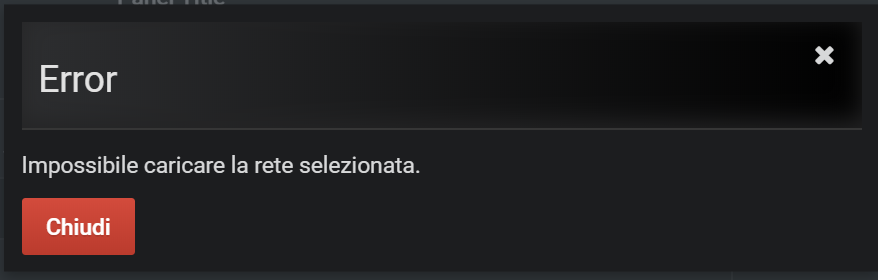
\includegraphics[scale=0.6]{./images/ErroreUpRete.png}
		 \caption{Messaggio di Errore caricamento Rete Bayesiana}	
		 \label{ErroreUpRete}
	\end{center}
\end{figure}



\pagebreak

\subsection{Selezione del Database}\label{SelectDB}

Una volta caricata una rete bayesiana (§\ref{ReteB}), al fine di collegare la stessa al flusso di monitoraggio, l'utente deve selezionare il Database contenente i dati da monitorare.\\
Tale operazione si articola in due passaggi fondamentali:
\begin{enumerate}
	\item \textbf{Passaggio 1:} L'utente seleziona, attraverso un menù a tendina, il database da usare come sorgente dati (Figura \ref{Sorgenti});
	\begin{figure}[H]
	\begin{center}
		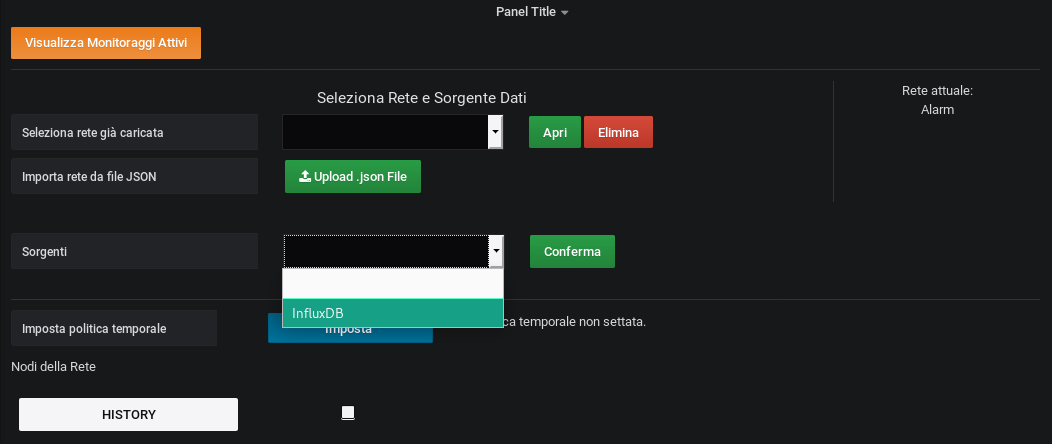
\includegraphics[scale=0.68]{./images/Sorgenti.png}
		 \caption{Elenco Database disponibili per il collegamento}	
		 \label{Sorgenti}
	\end{center}
	\end{figure}
	\item \textbf{Passagio 2:} L'utente conferma la propria scelta attraverso il pulsante \textbf{Conferma}, presente in Figura \ref{Sorgenti}.
\end{enumerate}
~\\
Al seguito della corretta selezione del Database da usare come sorgente dati l'utente verrà avvisato del buon esito dell'operazione da un messaggio di notifica (Figura \ref{NotificaSorgente}). 

\begin{figure}[H]
	\begin{center}
		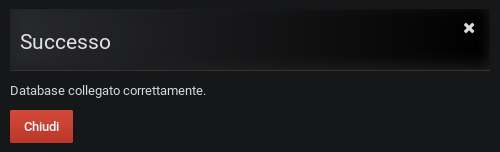
\includegraphics[scale=0.6]{./images/NotificaSorgente.png}
		 \caption{Notifica avvenuto collegamento Databse}	
		 \label{NotificaSorgente}
	\end{center}
\end{figure}

\pagebreak

\subsection{Collegamento Nodi al Flusso Dati}\label{Collegamento}

L'operazione di collegamento dei nodi della rete bayesiana al flusso dati è probabilmente la più articolata e dispendiosa del prodotto realizzato. Al fine di fornirne una spiegazione esaustiva ma al contempo intuitiva tale operazione verrà suddivisa in svariati passaggi:
~\\

\textbf{PREAMBOLO:} L'utente, a seguito del caricamento di una rete bayesiana (§\ref{ReteB}), visualizza la lista dei nodi di cui tale rete è costituita, tale situazione è presentata in Figura \ref{NodiRete}. Oltre al nominativo del nodo stesso viene visualizzata una checkbox che indica se il nodo in questione sia o meno collegato ad un flusso dati. Nel caso di nodo collegato viene visualizzato anche un pulsante \textbf{Scollega} attraverso cui è possibile scollegare il nodo dal flusso dati con un unico click.\\
Della lista di nodi visualizzata l'utente ha la possibilità di collegare ogni nodo, senza eccezioni, ad un flusso dati desiderato.
~\\

\textbf{PASSAGGIO 1:} L'utente clicca il nominativo del nodo che desidera collegare per accedere al \textbf{Pannello di Collegamento} (Figura \ref{PannelloNodo}), ove può configurare le necessarie impostazioni di collegamento per il nodo in esame.

\begin{figure}[H]
	\begin{center}
		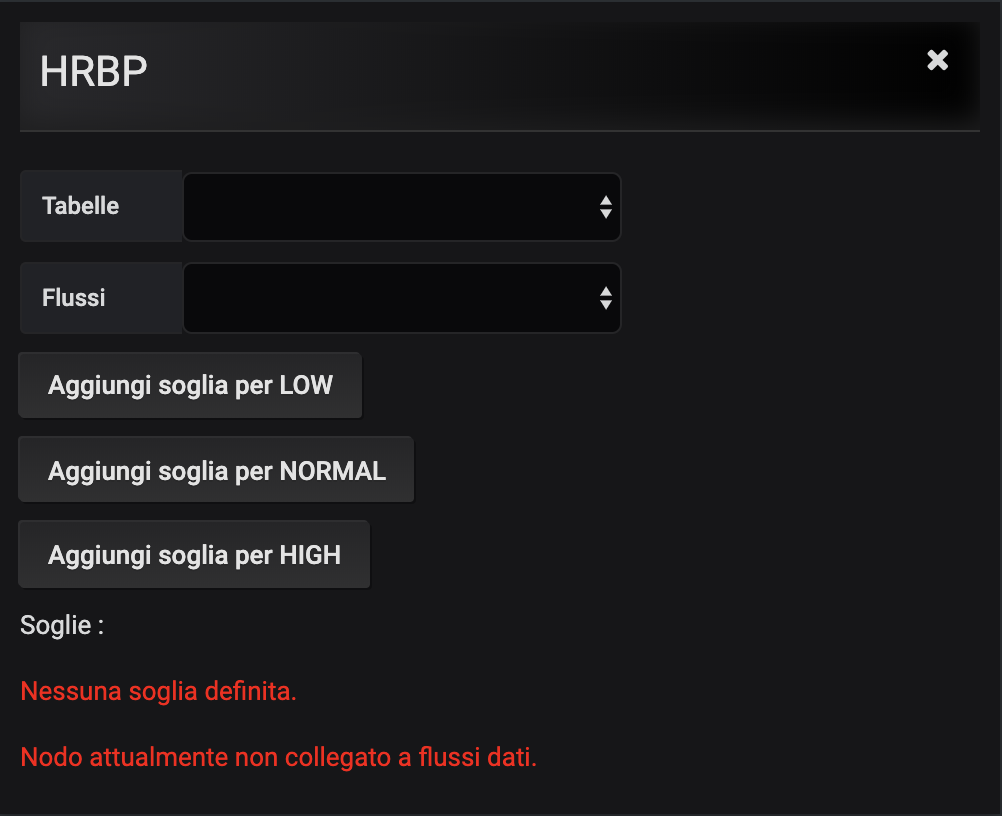
\includegraphics[scale=0.6]{./images/PannelloNodo.png}
		 \caption{Pannello di Collegamento del Nodo}	
		 \label{PannelloNodo}
	\end{center}
\end{figure}

\pagebreak

\textbf{PASSAGGIO 2:} Le prime impostazioni che l'utente è invitato a configurare riguardano la scelta della tabella, e del conseguente flusso dati (Figura \ref{PannelloNodo}), del database (selezionato in §\ref{SelectDB}). Tali impostazioni determinano univocamente lo specifico flusso dati di monitoraggio a cui l'utente collega il nodo della rete bayesiana.
~\\

\textbf{PASSAGGIO 3:} A questo punto l'utente deve configurare le soglie associate ad ogni possibile stato del nodo in esame. Tali soglie verranno verificate in sede di monitoraggio per associare un valore di evidenza al nodo della rete bayesiana in un dato istante.Possiamo suddividere questo passaggio in ultreriori cinque passi:
\begin{enumerate}
	\item L'utente seleziona \textbf{Aggiungi soglia} (pulsante presente in Figura \ref{PannelloNodo}) per aggiungere una soglia allo stato del nodo associato. È possibile aggiungere più soglie allo stesso stato;
	\item L'utente indica il valore numerico della soglia che sta definendo attraverso l'apposito campo dati visibile in Figura \ref{PannelloSoglie};
	\item L'utente seleziona, tramite la casella a scelta multipla, un valore tra i possibili: "<","<=",">" o ">=", per indicare la tipologia di soglia che sta configurando (Figura \ref{PannelloSoglie});
	\item Se lo desidera l'utente può etichettare la soglia come "critica" attraverso l'apposita checkbox (Figura \ref{PannelloSoglie}). In tal caso la verifica di tale soglia verrà fatta a prescindere dalla politica temporale delezionata in §\ref{policy};
	\item Se lo desidera l'utente può rimuovere una soglia attraverso il pulsante \textbf{Remove} presente in Figura \ref{PannelloSoglie}.
\end{enumerate}

\begin{figure}[H]
	\begin{center}
		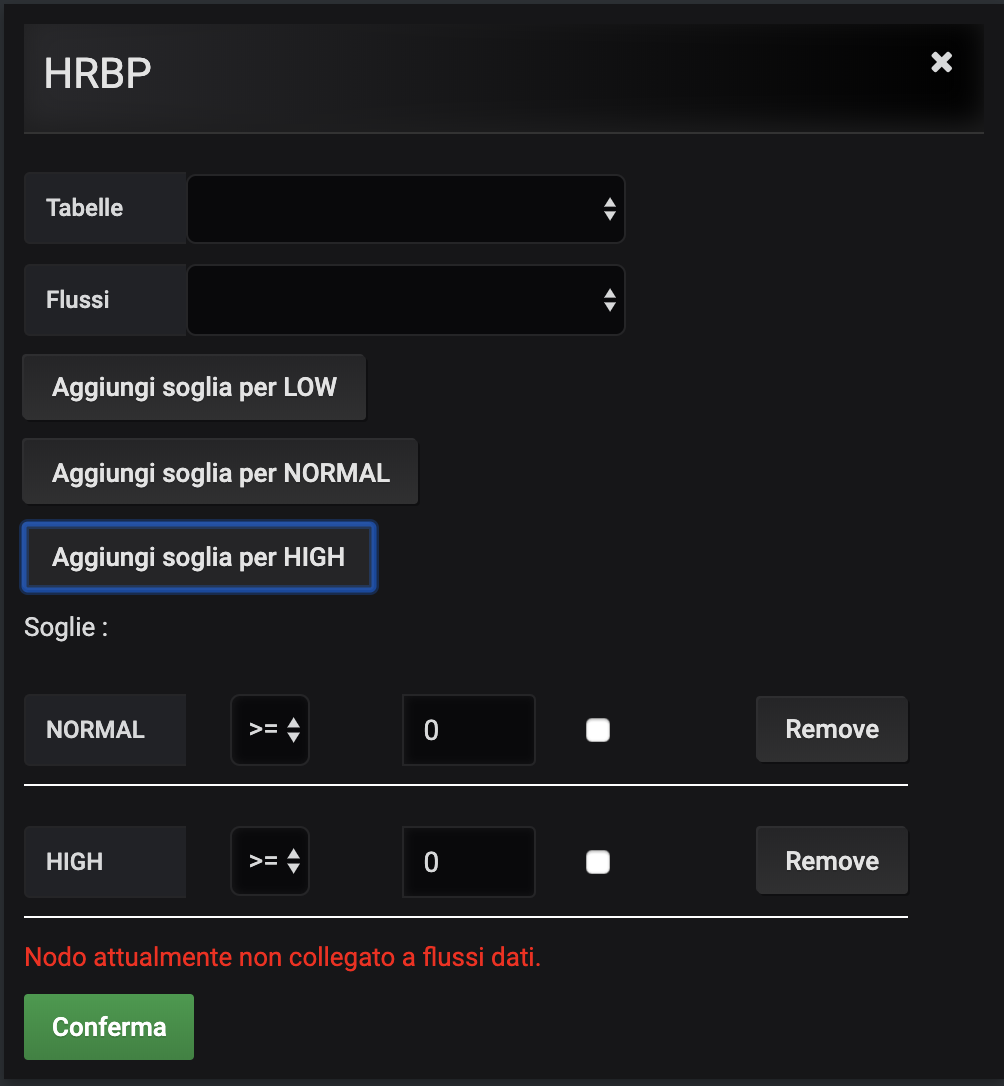
\includegraphics[scale=0.55]{./images/PannelloSoglie.png}
		 \caption{Pannello di Collegamento del Nodo con vista sulla definizione delle soglie}	
		 \label{PannelloSoglie}
	\end{center}
\end{figure}

\textbf{PASSAGGIO 4:} Infine l'utente deve confermate le proprie scelte di collegamento del nodo attraverso il pulsante \textbf{Conferma Collegamento} presente in Figura \ref{PannelloSoglie}.

~\\
A seguito del corretto collegamento del nodo al flusso dati l'utente verrà avvisato del buon esito dell'operazione da un messaggio di notifica (Figura \ref{NotificaCollegamento}).

\begin{figure}[H]
	\begin{center}
		
\includegraphics[scale=0.6]{./images/NotificaCollegamento.png}
		 \caption{Notifica di avvenuto collegamento del Nodo al flusso dati}	
		 \label{NotificaCollegamento}
	\end{center}
\end{figure}

L'utente visualizza inoltre, accanto al nodo in esame, la spunta sulla checkbox che ne indica lo stato di "Collegato al flusso dati" e il pulsante \textbf{Scollega Nodo} (Figura \ref{NodoCollegato}) per scollegare con un solo click il nodo al flusso dati.
 
 \begin{figure}[H]
	\begin{center}
		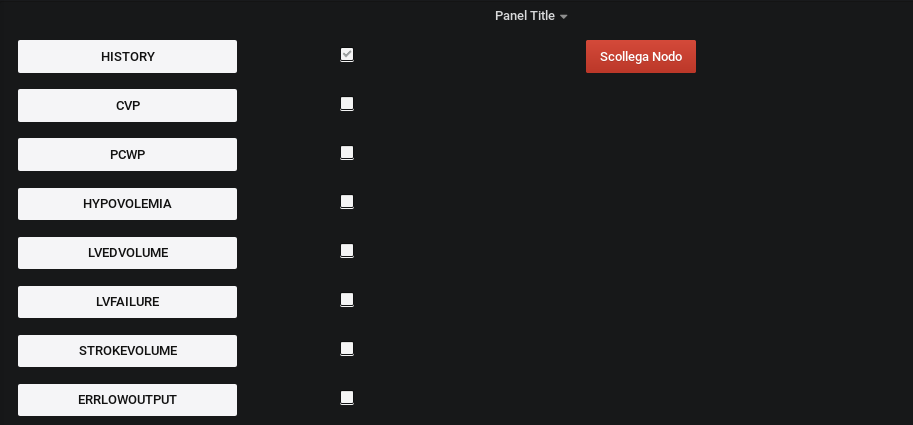
\includegraphics[scale=0.4]{./images/NodoCollegato.png}
		 \caption{Visualizzazione Nodo Collegato}	
		 \label{NodoCollegato}
	\end{center}
\end{figure}

\textbf{\textcolor{red}{ATTENZIONE}}: Nel caso in cui l'utente abbia commesso degli errori in fase di definizione delle impostazioni di collegamento l'operazione non va a buon fine e l'utente viene avvisato degli errori commessi da un messaggio di errore. Un esempio di tale situazione è fornito in Figura \ref{ErroreCollegamento}.

\begin{figure}[H]
	\begin{center}
		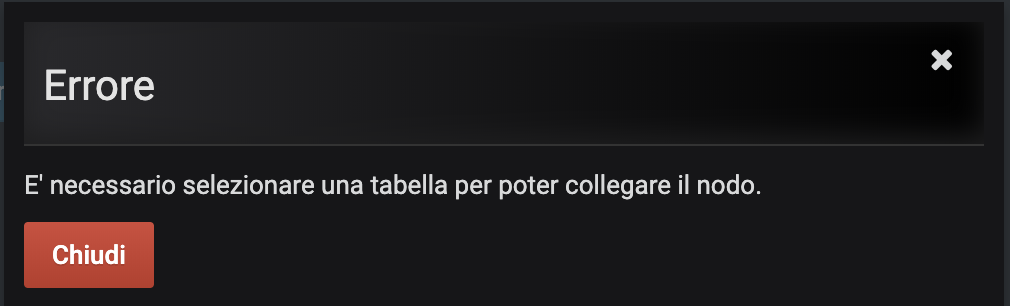
\includegraphics[scale=0.6]{./images/ErroreCollegamento.png}
		 \caption{Messaggio di Errore collegamento Nodo al flusso dati}	
		 \label{ErroreCollegamento}
	\end{center}
\end{figure}
 

\pagebreak

\subsection{Definizione di una Politica Temporale di Ricalcolo}\label{policy}

L'utente deve inoltre avere la possibilità di definire un Politica Temporale per il ricalcolo delle probabilità associate ai nodi delle rete in fase di monitoraggio.\\
Per poter effettuare questa operazione l'utente deve, come prima cosa, accedere al pannello per la definizione della politica temporale tramite il pulsante \textbf{Imposta} posizionato accanto alla label "Imposta politica temporale" (Figura \ref{Pannello}).\\
~\\
L'utente deve quindi configurare la politica temporale attraverso la compilazione dei tre campi dati: "Secondi", "Minuti" ed "Ore" presenti in Figura \ref{PannelloPolicy}. Attraverso questi campi è possibile deinire con precisione e semplicità la politica temporale, ovvero il temout ciclico per il ricalcolo delle probabilità in fase di monitoraggio.

\begin{figure}[H]
	\begin{center}
		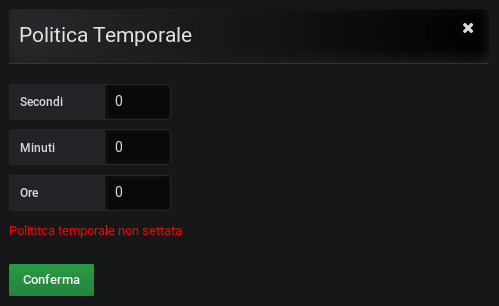
\includegraphics[scale=0.6]{./images/PannelloPolicy.png}
		 \caption{Pannello di configurazione della Politica Temporale}	
		 \label{PannelloPolicy}
	\end{center}
\end{figure} 

L'utente deve infine confermare le proprie scelte attraverso il pulsante \textbf{Conferma}, presente anch'esso in Figura \ref{PannelloPolicy}.
~\\
Al seguito della corretta definizione della politica temporale l'utente verrà avvisato del buon esito dell'operazione da un messaggio di notifica (Figura \ref{NotificaPolicy}). 

\begin{figure}[H]
	\begin{center}
		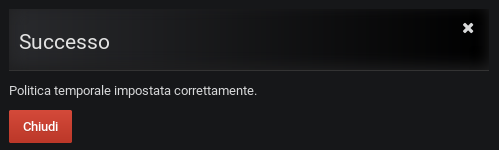
\includegraphics[scale=0.6]{./images/NotificaPolicy.png}
		 \caption{Notifica avvenuto collegamento Databse}	
		 \label{NotificaPolicy}
	\end{center}
\end{figure}

~\\
\textbf{\textcolor{red}{ATTENZIONE}}: Nel caso in cui l'utente abbia commesso degli errori in fase di compilazione dei campi dati l'operazione non va a buon fine e l'utente viene avvisato degli errori commessi da un messaggio di errore (Figura \ref{ErrorePolicy}). Nello specifico i campi dati \textbf{"Secondi"} e \textbf{"Minuti"} accettano numeri interi compresi tra 0 e 59, mentre il campo \textbf{"Ore"} deve essere compilato con numeri interi positivi.

\begin{figure}[H]
	\begin{center}
		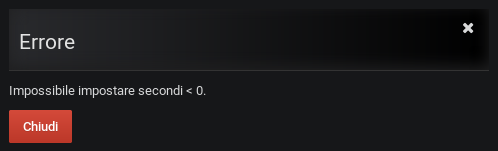
\includegraphics[scale=0.6]{./images/ErrorePolicy.png}
		 \caption{Messaggio di Errore configurazione Politica Temporale}	
		 \label{ErrorePolicy}
	\end{center}
\end{figure}



\pagebreak

\subsection{Selezione di una Rete Bayesiana Esistente}\label{SelezioneRete}

Oltre a poter caricare una rete attraverso l'upload di un file di definizione in formato \textit{JSON} (§\ref{ReteB}), l'utente ha anche la possibilità di selezionare una rete già caricata in precedenza. In questo caso verranno visualizzate nel pannello \textit{G\&B} la rete selezionata con le relative impostazioni di collegamento memorizzate.\\
L'operazione di selezione di una rete bayesiana esistente si articola in due semplici passaggi:
\begin{enumerate}
	\item \textbf{Passaggio 1:} L'utente seleziona, attraverso l'apposito menù a tendina visibile in Figura \ref{SelezioneReteImg}, una delle reti bayesiane memorizzate nel server;
	\item \textbf{Passaggio 2:} L'utente conferma il caricamento cliccando il pulsante \textbf{Apri}.
\end{enumerate}

\begin{figure}[H]
	\begin{center}
		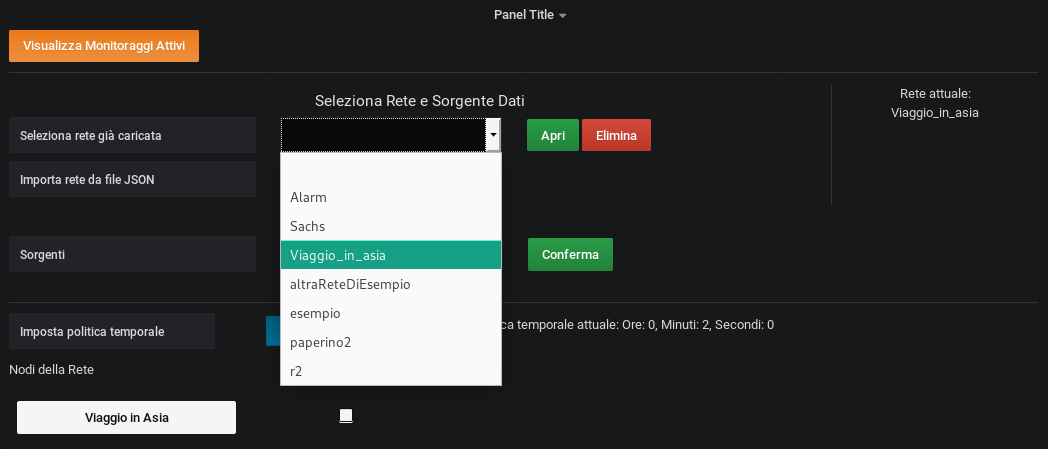
\includegraphics[scale=0.68]{./images/SelezioneRete.png}
		 \caption{Selezione di una Rete Bayesiana già Caricata}	
		 \label{SelezioneReteImg}
	\end{center}
\end{figure}

A seguito del corretto caricamento della rete bayesiana, l'utente verrà avvisato del buon esito dell'operazione da un messaggio di notifica (Figura \ref{NotificaSelezioneRete}). Inoltre, nel caso l'utente stesse visualizzando una diversa rete bayesiana prima della selezione, questa viene memorizzata nel server insieme alle sue eventuali impostazioni di collegamento.

\begin{figure}[H]
	\begin{center}
		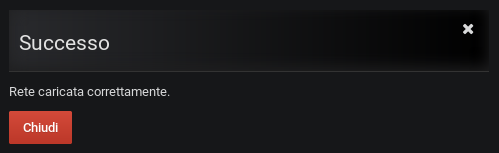
\includegraphics[scale=0.6]{./images/NotificaSelezioneRete.png}
		 \caption{Notifica di Avvenuto Caricamento della Rete Bayesiana}	
		 \label{NotificaSelezioneRete}
	\end{center}
\end{figure}





\pagebreak

\subsection{Eliminazione di una Rete Bayesiana}\label{EliminazioneRete}

Accanto alla selezione di una rete bayesiana già caricata (§\ref{SelezioneRete}), esiste anche l'operazione speculare di rimozione di una rete bayesiana memorizzata nel server.\\
Anche questa operazione consta di due passaggi, di cui il primo assolutamente analogo all'operazione precedente:
\begin{enumerate}
	\item \textbf{Passaggio 1:} L'utente seleziona, attraverso l'apposito menù a tendina visibile in Figura \ref{SelezioneReteImg}, una delle reti bayesiane memorizzate nel server;
	\item \textbf{Passaggio 2:} L'utente conferma l'eliminazione della rete attraverso il pulsante \textbf{Elimina}.
\end{enumerate}

A seguito della corretta rimozione della rete bayesiana, l'utente verrà avvisato del buon esito dell'operazione da un messaggio di notifica (Figura \ref{NotificaRimozioneRete}). La rete in questione, insieme alle relative impostazioni di collegamento, verrà rimossa sia dal pannello che dal server.

\begin{figure}[H]
	\begin{center}
		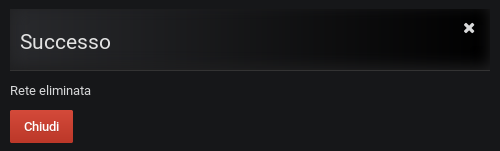
\includegraphics[scale=0.6]{./images/NotificaRimozioneRete.png}
		 \caption{Notifica di Avvenuta Rimozione della Rete Bayesiana}	
		 \label{NotificaRimozioneRete}
	\end{center}
\end{figure}

\textbf{\textcolor{red}{ATTENZIONE}}: Nel caso in cui l'utente abbia scelto di eliminare una rete al momento sotto monitoraggio attivo l'operazione non va a buon fine e l'utente viene avvisato di tale risultato da un messaggio di errore (Figura \ref{ErroreDeleteNet}).

\begin{figure}[H]
	\begin{center}
		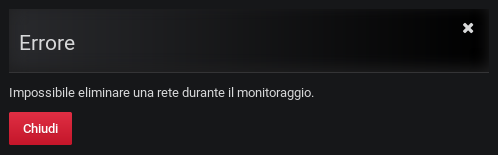
\includegraphics[scale=0.6]{./images/ErroreDeleteNet.png}
		 \caption{Messaggio di Errore Eliminazione di una Rete Bayesiana}	
		 \label{ErroreDeleteNet}
	\end{center}
\end{figure}


\pagebreak